\documentclass[a4paper,landscape]{standalone}
\usepackage{graphicx} % Required for inserting images
\usepackage{verbatim}

\title{compilers principles tikz}
\author{lhm}
\date{September 2023}

%\def\pgfsysdriver{pgfsys -dvipdfmx.def}
\usepackage{tikz}
\usetikzlibrary{graphs} 
%\usetikzlibrary{shapes,arrows}
\tikzstyle{arrow}=[draw,-latex]
\tikzset{
cir/.style ={
circle, %circle节点
minimum width =30pt ,
minimum height =30pt,
draw=black}
}


\begin{document}

%\maketitle


\vspace{20ex}
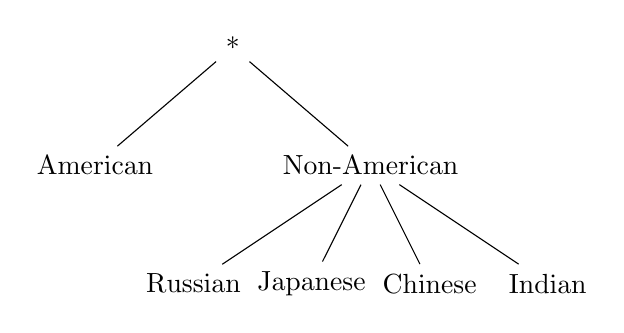
\begin{tikzpicture}
    \node at(0,0) {*}
    child {node at(-1,0){American}
        }
    child {node at(1,0) {Non-American}
            child{node {Russian}}
            child{node {Japanese}}
            child{node {Chinese}}
            child{node {Indian}}
        }
    ;
\end{tikzpicture}

\end{document}

\begin{comment}
%nation
\node at(0,0) {*}
child {node at(-1,0){American}
    }
child {node at(1,0) {Non-American}
        child{node {Russian}}
        child{node {Japanese}}
        child{node {Chinese}}
        child{node {Indian}}
    }
;
\end{comment}

\begin{comment}
%zip code
\node at(0,0) {*}
child {node at(-1,0){130**}
        child{node {13053}}
        child{node {13068}}
    }
child {node at(1,0) {148**}
        child{node {14850}}
        child{node {14853}}
    }
;
\end{comment}

\begin{comment}
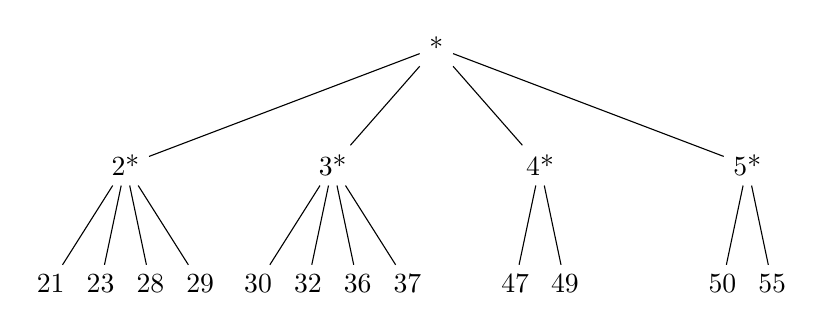
\begin{tikzpicture}[sibling distance=18pt]
    %age
    \node at(0,0) {*}
    child {node at(-3,0) {2*}
            child{node {21}}
            child{node {23}}
            child{node {28}}
            child{node {29}}
        }
    child {node at(-1,0) {3*}
            child{node {30}}
            child{node {32}}
            child{node {36}}
            child{node {37}}
        }
    child {node at(1,0) {4*}
            child{node {47}}
            child{node {49}}
        }
    child {node at(3,0) {5*}
            child{node {50}}
            child{node {55}}
        }
    ;
\end{tikzpicture}
\end{comment}

\begin{comment}
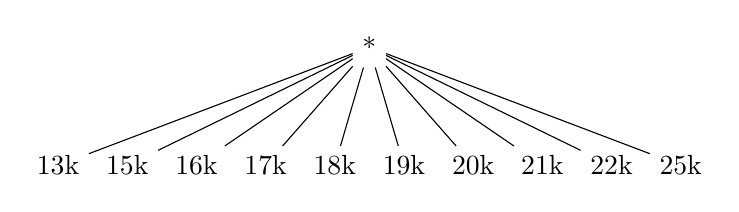
\begin{tikzpicture}[sibling distance=25pt]
    %salary
    \node at(0,0) {*}
    child {node {13k}}
    child {node {15k}}
    child {node {16k}}
    child {node {17k}}
    child {node {18k}}
    child {node {19k}}
    child {node {20k}}
    child {node {21k}}
    child {node {22k}}
    child {node {25k}}
    ;
\end{tikzpicture}
\end{comment}